\documentclass{beamer}
\usetheme{default}
\def\d{{\rm d}}
\begin{document}

\begin{frame}{Atomic Orbitals}

Atomic wavefunctions can be written as:
\[
    \psi_{nlm}({\bf x}) = R_{nl}(r) Y_{lm}(\Omega)
\]
we plot $| \psi_{nlm}({\bf x})|^2$ for Radium (Z=88) with electronic
configuration: $1s^2 2s^2 2p^6 3s^2 3p^6 3d^{10} 4s^2 4p^6 5s^2 4d^{10}
5p^6 4f^{14} 5d^{10} 6s^2 6p^6 7s^2$

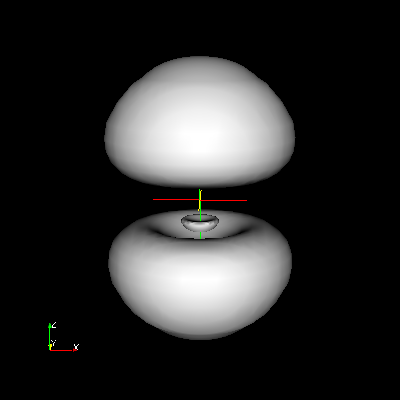
\includegraphics[width=1in]{../img/orbital_n6l1m0.png}
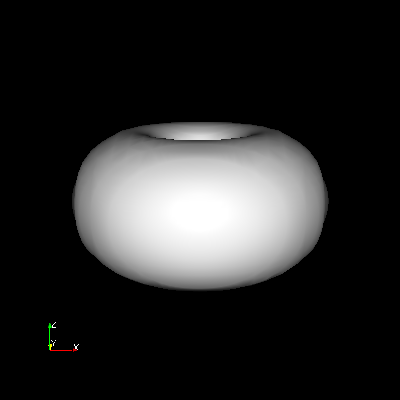
\includegraphics[width=1in]{../img/orbital_n5l2m2.png}
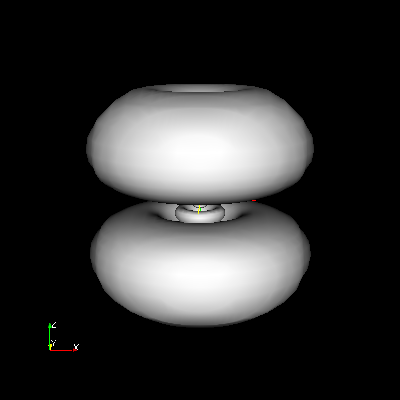
\includegraphics[width=1in]{../img/orbital_n5l2m1.png}
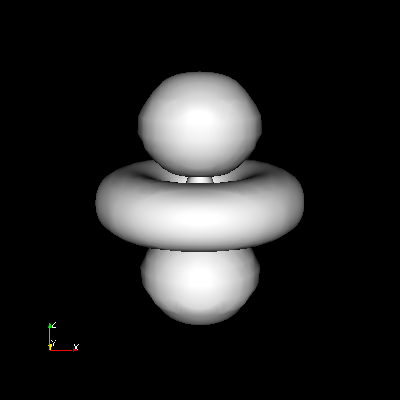
\includegraphics[width=1in]{../img/orbital_n5l2m0.png}

From left to right $(n l m)$: 610, 522, 521, 520

\end{frame}

\begin{frame}{More Examples Atomic Orbitals}

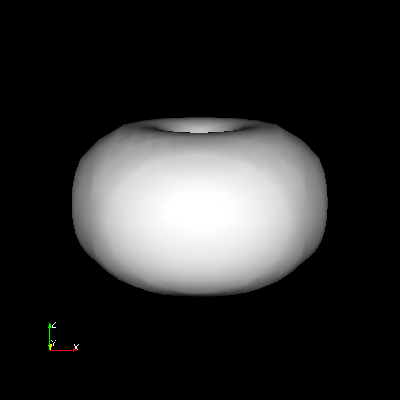
\includegraphics[width=1in]{../img/orbital_n3l2m2.png}
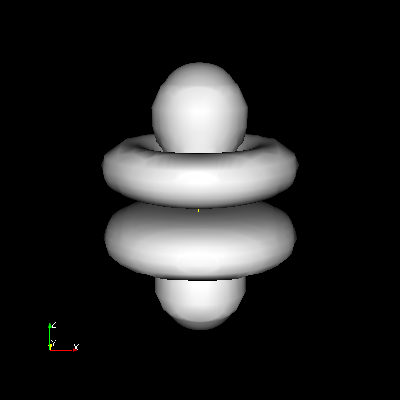
\includegraphics[width=1in]{../img/orbital_n4l3m0.png}
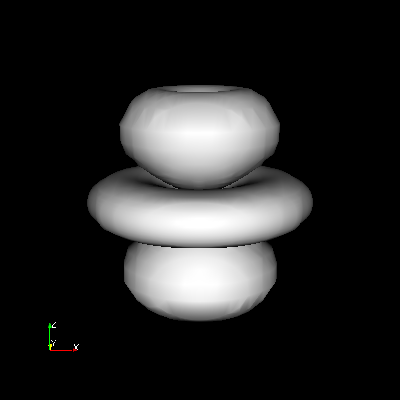
\includegraphics[width=1in]{../img/orbital_n4l3m1.png}
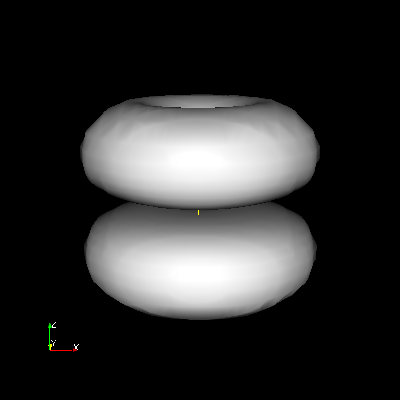
\includegraphics[width=1in]{../img/orbital_n4l3m2.png}

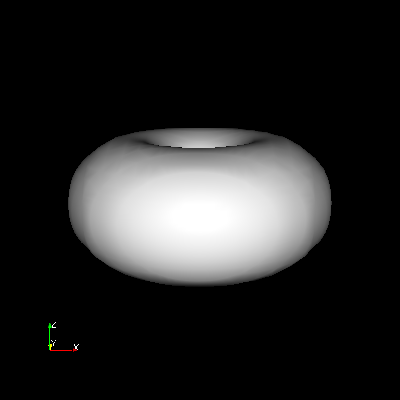
\includegraphics[width=1in]{../img/orbital_n4l3m3.png}
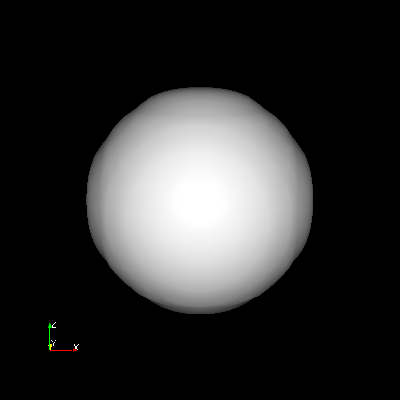
\includegraphics[width=1in]{../img/orbital_n5l0m0.png}
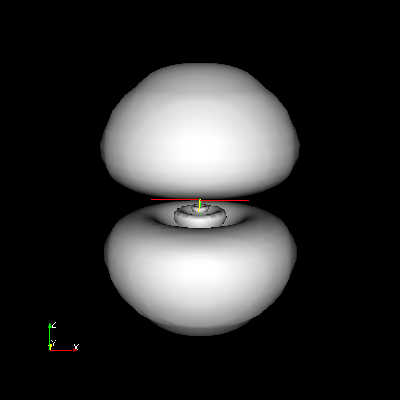
\includegraphics[width=1in]{../img/orbital_n5l1m0.png}
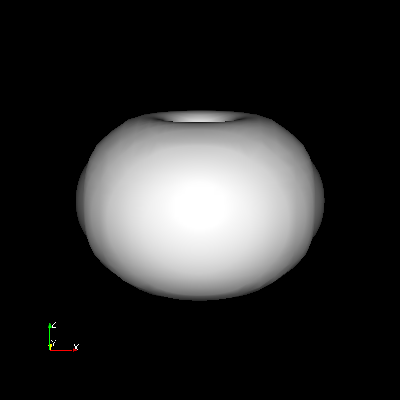
\includegraphics[width=1in]{../img/orbital_n5l1m1.png}

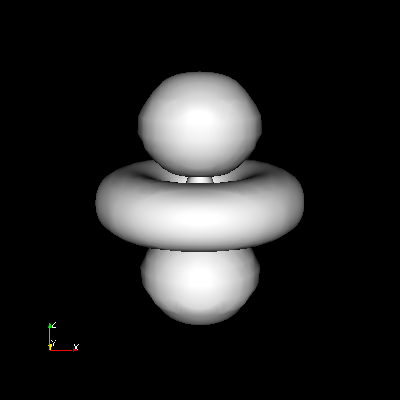
\includegraphics[width=1in]{../img/orbital_n5l2m0.png}
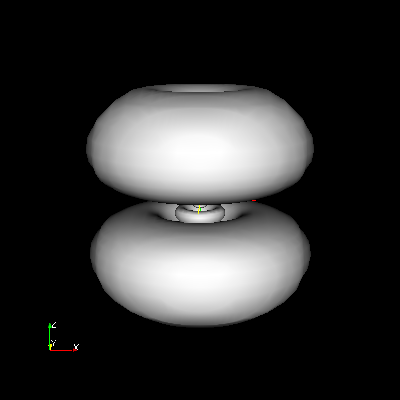
\includegraphics[width=1in]{../img/orbital_n5l2m1.png}
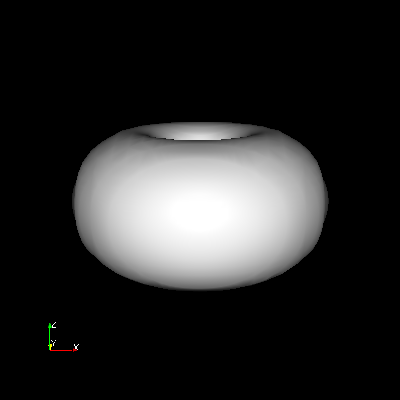
\includegraphics[width=1in]{../img/orbital_n5l2m2.png}
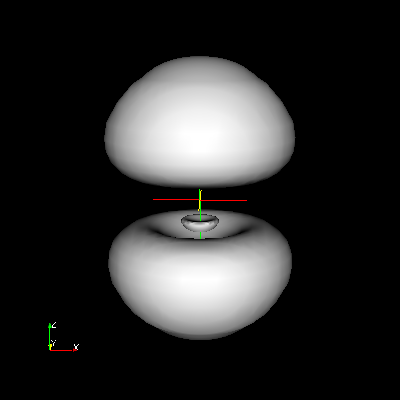
\includegraphics[width=1in]{../img/orbital_n6l1m0.png}


\end{frame}

\begin{frame}{Details}

We are solving the Hartree-Fock equations:
\[
    \left(-{1\over 2} \nabla^2 -{Z\over |{\bf x}|}
    +
    \int {\sum_{j=1}^Z|\psi_j({\bf y})|^2\over|{\bf x}-{\bf y}|}
            \d^3 y\right)\psi_i({\bf x}) +
\]
\[
    - \sum_{j=1}^Z\int {\psi_i({\bf y})\psi_j^*({\bf y})\over|{\bf x}-{\bf y}|}
            \d^3 y\,\,\psi_j({\bf x})
    =
    \epsilon_i \psi_i({\bf x})
\]
(where $Z$ is the atomic charge, ${\bf x}$, ${\bf y}$ are 3D coordinates and
$\psi_i({\bf x})$ are atomic orbitals) in spherical symmetry. After
manipulation, they become (for closed shell atoms):

\[
    -{1\over2} P_{nl}''(r) +
        \left({l(l+1)\over 2r^2} -{Z\over r} + V_H(r)\right)P_{nl}(r) +
\]
\[
            -\sum_{n'l'}
                f_{n'l'}
                \sum_{k=|l-l'|}^{k=l+l'}
                {1\over2}\begin{pmatrix} l & k & l' \\ 0 & 0 & 0 \end{pmatrix}^2
                \int
                {r_{<}^k\over r_{>}^{k+1}}
                P_{nl}(r')
                P_{n'l'}(r')
                \d r'\,
                    P_{n'l'}(r)
        =
\]
\[
        = \epsilon_{nl} P_{nl}(r)
\]


\end{frame}

\begin{frame}{Weak Formulation}

\[
    \int_0^\infty \left( {1\over2} u'(r) v'(r) +
        \left({l(l+1)\over 2r^2} -{Z\over r} + V_H(r)\right)u(r)v(r)
            \right) \d r+
\]
\[
            -\sum_{n'l'}
                2(2l'+1)
                \sum_{k=|l-l'|}^{k=l+l'}
                {1\over2}\begin{pmatrix} l & k & l' \\ 0 & 0 & 0 \end{pmatrix}^2
                R^k(v, n'l', u, n'l')
        =
\]
\[
        = \epsilon \int_0^\infty u(r)v(r)\d r
\]

$R^k(a, b, c, d)$ is a Slater integral, $V_H(r)$ is a Hartree potential.
The solution $u$ is related to $R(r)$ from the first slide by:

\[
    u(r) = rR(r)
\]

\end{frame}

\end{document}
